\chapter{Radio Propagation Simulation} \label{ch:radio_propagation}

\section{Introduction}
%introduce the section and what will be discussed here
The simulation software is broken down into three main components, the radio wave propagation model, the scene model, and the ray tracing engine. The wave propagation model is a collection of equations that describe the physical phenomena that affect the propagation when represented by rays. The model used is based upon classical geometric optics to work with the ray tracing engine. The scene model is comprised of a 3D environment in order to define the physical rotor blade surface. The receiver and transmitter will also be defined in the same environment with simulated characteristics to match real life conditions. The ray tracing engine uses recursive execution described in \cite{Whitted1979}, replacing cameras and lights for receivers and transmitters respectively in a three dimensional environment.

\section{Radio Propagation Model}
%define the math behind the physical laws that are simulated within the simulation
The propagation model defined in this project is based on the following physical phenomena; free-space path loss, reflection, and the doppler effect. They are all formally established models described in full in \cite{Bertoni1999}, \cite{Parsons2000}, and \cite{Willis2005}. Although several effects are described within the model several were left out to simplify the computation due to the overhead of implementation in 3D space and because of the assumptions made about the scene model.

\subsection{Free-Space Path Loss}
%describe path loss
Free-Space path loss is calculated using the Friis transmission and is incorporated into the model by keeping track of the distance a ray travels and adjusting its power is

%FSPL formula
\begin{equation}
	 P_r = G_r G_t P_t \left (\frac{\lambda}{4\pi R}\right)^2
	 \label{eqn:FSPL}
\end{equation}

%formula description
where $P_r $ is the power at the receiver, $P_t$ is the power at the transmitter, $G_r$ and $G_t$ are the antenna gains, 
$\lambda$ is the wavelength, and $R$ is the distance between the receiver and transmitter antennas. In the simulations described in this paper, $G_r$ and $G_t$ are assumed to have a value of 1.

\subsection{Reflection}

\subsubsection{Specular Reflection}
In the case of a perfect reflection the angle of the reflection is calculated by

%Spec formula
\begin{equation}
	\theta_r = \cos^{-1}(\vec{n} \bullet (-\vec{d_i}))
	\label{eqn:spec}
\end{equation}

%formula description
where $\theta_r$ is the angle of the reflected ray, $\vec{n}$ is the normal vector to the surface, and $\vec{d_i}$ is the direction vector of the incident ray.

\subsubsection{Reflection Loss}
Power loss due to surface reflection is described through the following coefficient

%Reflection loss formula
\begin{equation}
	\Gamma = \frac{\cos(\theta_i) - \sqrt{\varepsilon}\cos(\theta_t)}{\cos(\theta_i) + \sqrt{\varepsilon}\cos(\theta_t)}
	\label{eqn:RL}
\end{equation}

%formula description
where $\theta_i$ is the angle of incidence with the object's surface normal, $\varepsilon$ is the dielectric constant for that surface, and $\theta_t$ is the angle of refraction as described by Snell's law

\begin{equation}
	\theta_t = \sin^{-1}\left(\frac{\sin(\theta_i)}{\sqrt{\varepsilon}} \right)
	\label{eqn:snell}
\end{equation}

The final reflected power is then

\begin{equation}
	P_{reflected} = P_i|\Gamma|
	\label{eqn:reflected_power}
\end{equation}

%reflection power loss description
where $P_i$ is the incident power before reflection loss.

\subsubsection{Diffuse Reflection}
A perfect diffuse reflection, also known as Lambertian reflection, will reflect rays in all directions in a uniform hemisphere \cite{Sizun2005}. The hemisphere is centered at the point the ray hits, producing rays away from the surface. To approximate a particular type of surface the rays power is attenuated by the surface's bi-directional reflectance distribution function (BRDF) \cite{Suffern2007}, \cite{Pharr2010}, \cite{Glassner1995}. There are several ways of calculating the BRDF, but the simplest is the Phong BRDF which will be used in this ray tracing implementation \cite{Phong:1998:ICG:280811.280980}. This method for the BRDF is regularly used in the rendering of computer graphics to simulate the reflection of light off surfaces and combines the diffuse and specular components. Since this was not designed for the longer wavelengths used in RF communications, an assumption is made about surface features. Where features relevant to light waves,  produce a reflectance distribution similar for this application. 

%The BRDF parameters were then selected to be frequency independent to form a plausible reflectance distribution for the physical effects.

%multipath fading
\subsection{Fading}
The transmitted signal power experiences fading described by

\begin{equation}
	F = cos\left(2\pi \frac{d}{c} + t_0\right)
	\label{eqn:fading_coeff}
\end{equation}

where $F$ is the fading coefficient, $d$ is the total distance the particular ray has traveled, $c$ is the speed of light, and $t_0$ is the starting time of the current frame. The power can then be calculated using

\begin{equation}
	P_{faded} = PF
	\label{eqn:power_faded}
\end{equation}

where $P_{faded}$ is the adjusted power due to fading and $P$ is the signal power. The superposition of each ray's faded power becomes the received signal.

\subsection{Doppler Effect}
%define doppler effect
The Doppler effect is characterized by

%Doppler formula
\begin{equation}
	f = \left ( \frac{c + v_r}{c + v_s} \right ) f_0
	\label{eqn:formalDop}
\end{equation}

It is assumed that both the receiver and the transmitter are not moving therefore, the only Doppler imparted on the signal will be from the rotation of the blades. The associated Doppler is calculated using

%formula for doppler on the rotor blade.
\begin{equation}
	f = f_0 + \frac{v_t + v_r}{\lambda} %reradiated after reflection
	\label{eqn:observedShift}	
\end{equation}

where $f_0$ is the initial transmitted frequency, $\lambda$ is the wavelength, $v_t$ is the velocity in the direction of the transmitter, and $v_r$ is the velocity in the direction of the reflection. This is similar to the Bistatic radar equation for Doppler, but since the reflection is not guaranteed to be toward the receiver we calculate the doppler as it makes contact with the surface and as it is re-radiated according the blades direction of travel.

\begin{equation}
	\lambda = \frac{c}{f_0}
	\label{eqn:wavelength}
\end{equation}

where $\lambda$ is the wavelength of the transmitted signal based off of the speed of light $c$ and its initial frequency $f_0$

\begin{equation}
	v_t = r \omega_r (\vec{d_p} \bullet \vec{d_t})
	\label{eqn:v_t}
\end{equation}

%formula description
where $r$ is the radius along the length of the blade where the reflection occurs. $\omega_r$ is the angular velocity of the rotor. $\vec{d_p}$ is the normalized vector that is perpendicular to the rotor in its direction of travel and $\vec{d_t}$ is the normalized vector that is in the direction of the transmitted ray.

\begin{equation}
	v_r = r \omega_r (\vec{d_p} \bullet \vec{d_r})
	\label{eqn:v_r}
\end{equation}

where $\vec{d_r}$ is the normalized vector that is in the direction of the reflected ray.

\section{Scene Model}
% describe what the scene model is and how it will fit in to the ray tracer and the 3d setting
The scene model is the 3D environment in which the physical objects are placed. 
The model is comprised of three types of objects; the rotor blades, transmitter and receiver. The rotor blade is the most complex object due to its airfoil shape. The transmitter is a point source that projects the rays into the scene, and the receiver is described in a similar fashion with a surrounding boundary layer. There are no other objects within the scene. This is because the effect of the rotor on the received signal is analyzed for defining characteristics without outside variables.

\subsection{Rotor Blade}
%go over the shape of the blade
The rotor blade is the most complex object within the scene, due to its airfoil shape. The airfoil shape is designed to produce lift for the helicopter, and designing one is outside the scope of this project. Fortunately, there are databases that provide real helicopter airfoil designs in x,y coordinates. This data forms a 2D cross-section of the airfoil shape that will be extruded into the length of the rotor blade. Figure \ref{fig:airfoil} shows the airfoil cross-section that will be used to create the rotor surface. 

%figure of 2D airfoil
\begin{figure}
	\begin{center}
		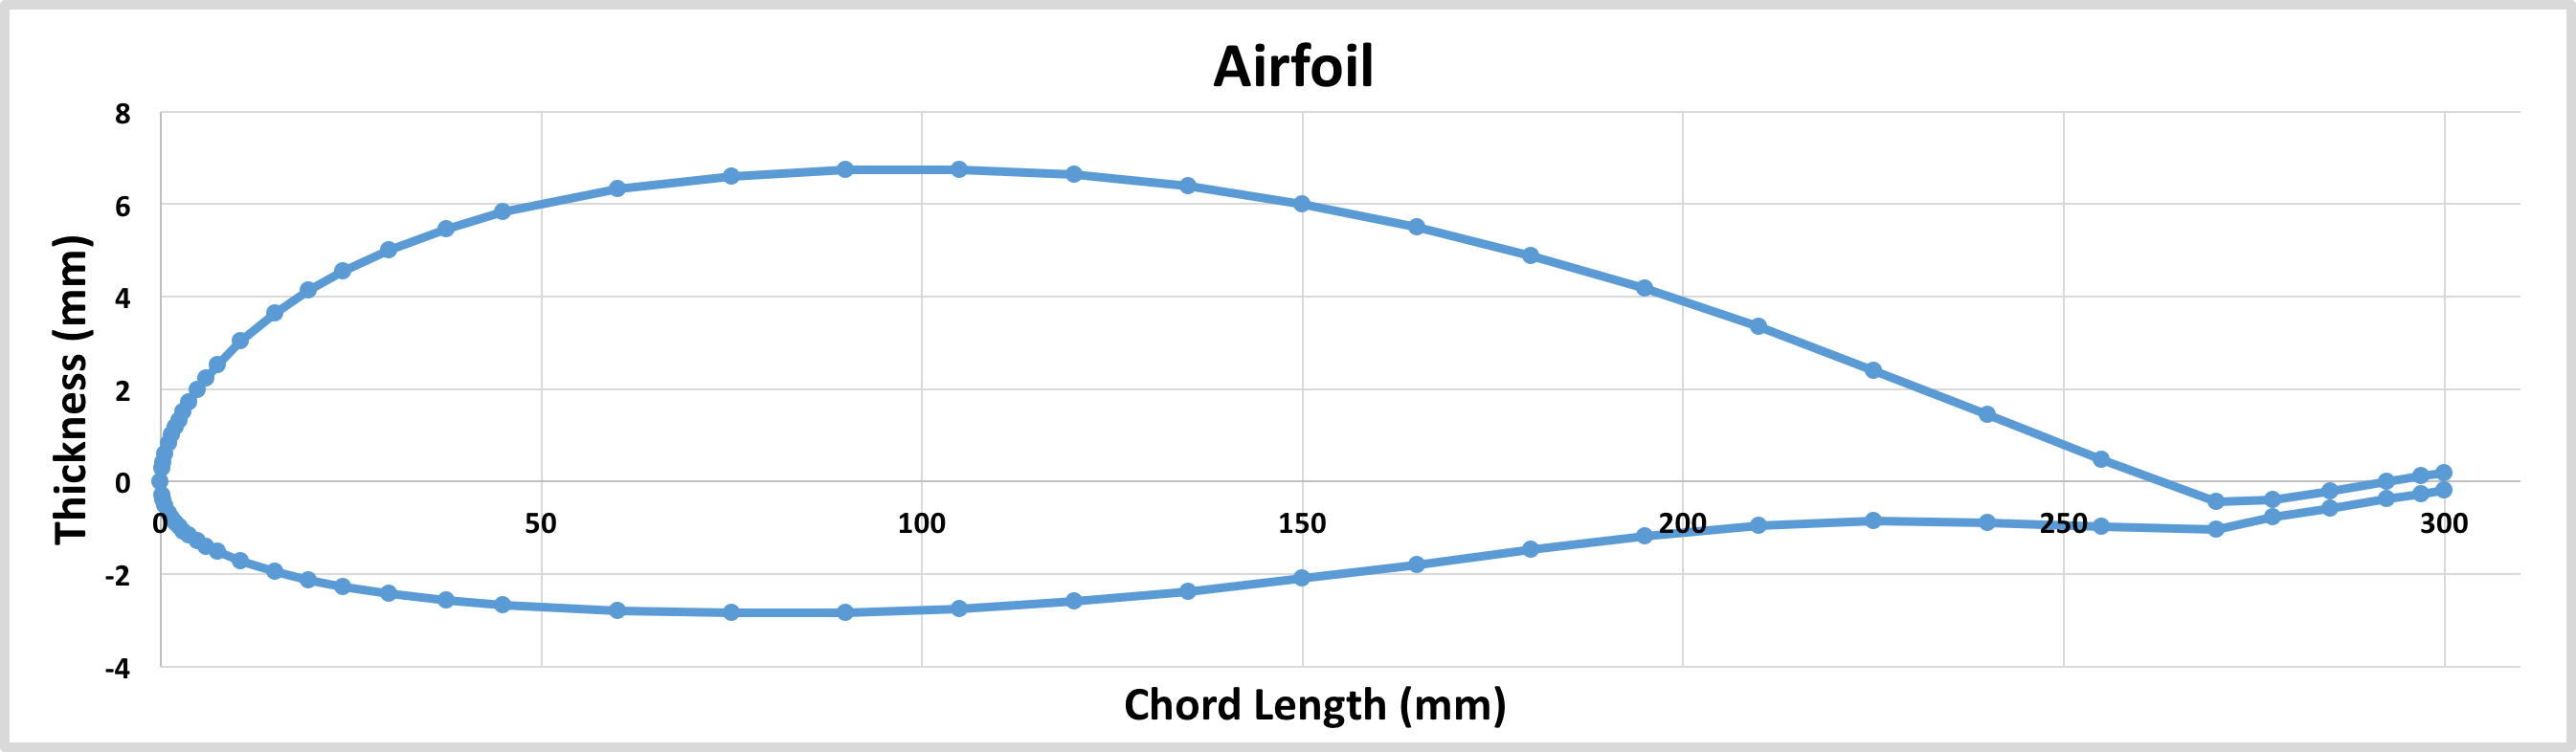
\includegraphics[width=15cm]{images/radio_propagation/2d_airfoil.png}
		\caption{Airfoil Cross-Section}
		\label{fig:airfoil}
	\end{center}
\end{figure}

%go over how it is formed and the tessellation code
The 2D airfoil sections will form the ribs of the rotor blade but the surface of the blade will be made up of primitive surfaces to approximate the curved airfoil shape. The primitive shapes are triangles that span between the ribs and go around to cover the surface. This was done using a lightweight mesh generation method using a priori knowledge of the blade's shape. The designed algorithm, located in \ref{class_blade__surface_a160959f632ad73eff846aeea81aa84ae} $create\_surface()$ method, takes advantage of the object's uniform structure in 2D. The surface normals are then adjusted to match the correct directionality. Figure \ref{fig:tessilation} shows the created surface for the rotor blade that will be used in the scene.

%figure of tessilation
\begin{figure}
	\begin{center}
		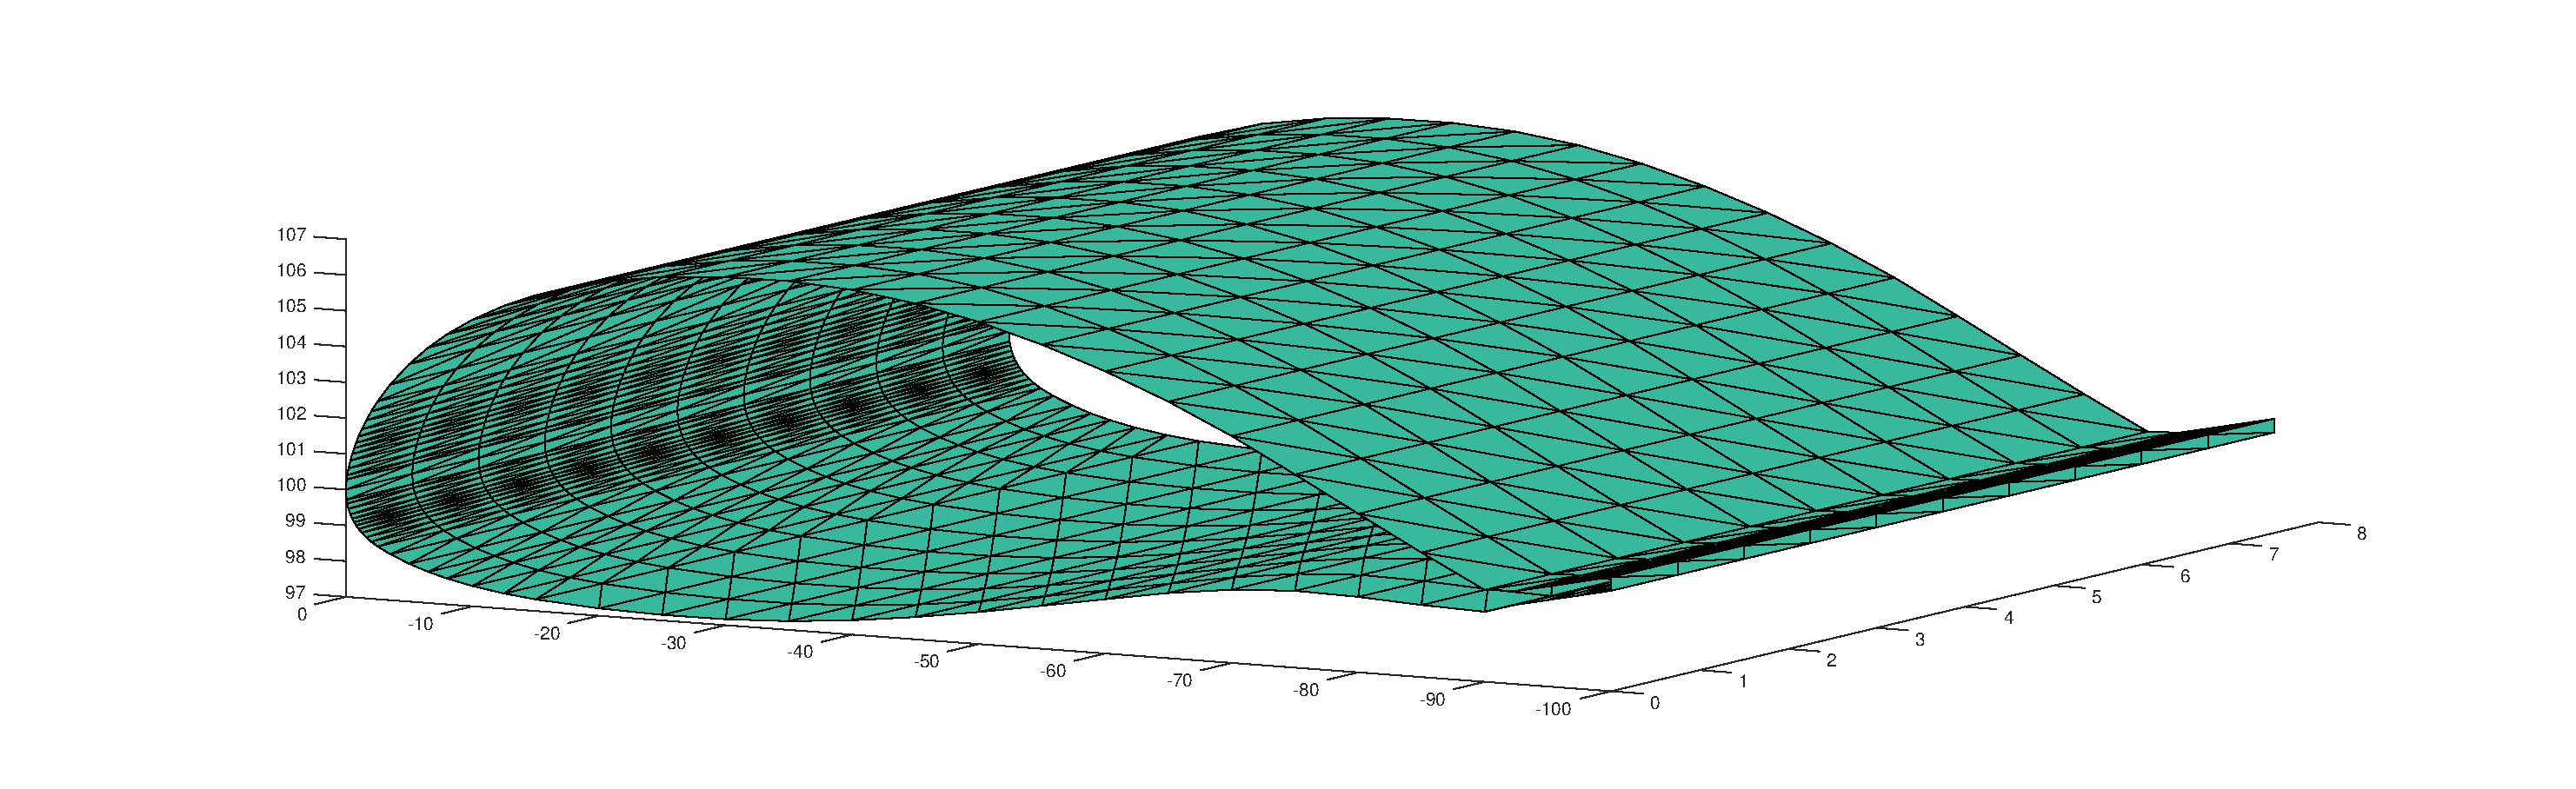
\includegraphics[width=15cm]{images/radio_propagation/blade_surface_tesselation.eps}
		\caption{Blade Surface Tessilation}
		\label{fig:tessilation}
	\end{center}
\end{figure}

%modular parameters
All aspects of the rotor blade are parameterized. Starting with the airfoil shape, which is defined by a set of 2D coordinates. The length and the number of rib sections can be configured along with the number of blades and corresponding altitude. As well as the RPM. This allows the scene to replicate any type of rotor configuration and position it at a specific altitude.

\subsection{Transmitter}
%point source transmitter casting rays in specific direction
The transmitter is modeled as a point source, this means that all the radio waves are projected from this point into the scene. It is assumed that the transmitter is located on the ground within the x,y plane in relationship to the rotor blades. The transmitter is configured with a center frequency and is assumed to produce a tone at that frequency. Therefor, the signal produced has no inherent modulation applied to it.
%direction creation
Being that the transmitter is emitting radio waves into a 3D space, it is assumed to be transmitting in an omnidirectional fashion. But because the rotor and the receiver are the only two other objects within the scene, radio waves will only be propagated in their direction. This limitation allows for a higher concentration of rays to be casted, resulting in a higher resolution picture that eliminates computational overhead for the tracing engine. Figure \ref{fig:transmitter_direction} shows the rays, in blue, casted only in the vicinity of the rotor blade and receiver.

%figure of transmitter direction
\begin{figure}
	\begin{center}
		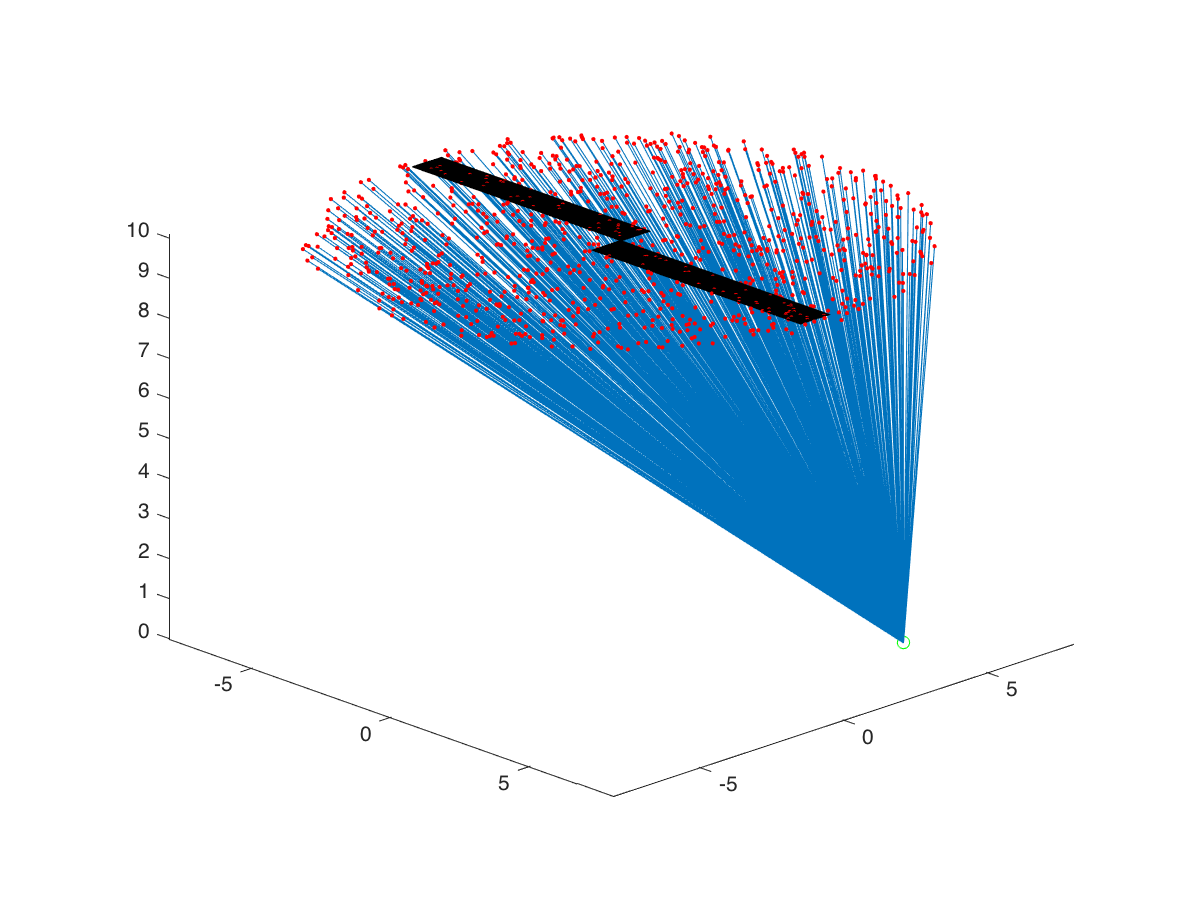
\includegraphics[width=15cm]{images/radio_propagation/transmitted.eps}
		\caption{Transmitter Rays}
		\label{fig:transmitter_direction}
	\end{center}
\end{figure}

\subsection{Receiver}
%physical receiver dimensions and antenna chars
The receiver object is modeled as a point in 3D space with a surrounding boundary layer in the shape of a sphere. This is because the receiver is assumed to have an omnidirectional antenna which will receive radio waves from all directions uniformly. The receiver will record any ray that hits the boundary layer within each frame of the simulation to create a sample of data at that instance in time.
%processing in each frame
The sample is produced using superposition of all the rays that are acting on the receiver at that instance in time which are then extrapolated to produce a clear result.
%realism
The receiver is configurable allowing the user to set a desired center frequency along with the sampling rate of the simulated hardware. The sampling rate will determine several simulation parameters in the ray tracer due to the need to associate this rate with the change in the rotor position for the next frame. The consequence of this is that increasing the sample rate will produce higher resolution results but, will increase the computational overhead of the simulation.

\section{Ray Tracing}
%describe the core tracing engine and describe the flow of the program
The ray tracing simulation is conducted in the Monte Carlo fashion acting on the scene and propagation models. This method of raytracing is established for creating realistic images in \cite{Suffern2007}, \cite{Pharr2010}. The simulation is performed over successive iterations. Each iteration is a discrete element called a frame and each frame will be updated to represent the change in the position of the rotor blade.

\subsection{Computation}
%flow of the program
The ray tracing engine first sets up the environment, creating the surfaces and placing the objects in the scene. Then the number of frames that will be computed. The number of frames is determined by the number of rotations that the rotor makes within the simulation, the speed of the rotor in RPM and the sampling frequency of the receiver defined before the beginning of the simulation. This is described by

%frame rates equation
\begin{equation}
	Frames = \frac{60  f_s}{RPM} Rev
	\label{eqn:frames}
\end{equation}

where $Frames$ is the number of frames that will be computed in the simulation, $f_s$ is the sampling frequency of the receiver, $RPM$ is the revolutions per minuet of the rotor, and $Rev$ is the number of revolutions that the rotor makes in the simulation.

In each frame a set number of rays are casted into the scene in a uniformly distributed circle in the direction of the rotor and receiver using

%uniform disk equation
\begin{equation}
	v_{ray} = \begin{bmatrix}
			x \\
			y \\
			z \\
	\end{bmatrix}
	= \begin{pmatrix}
			\sqrt{r} \cos{\theta_u}  + d_x\\
			\sqrt{r} \sin{\theta_u}  + d_y \\
			d_z \\
	\end{pmatrix}
	\label{eqn:disk}
\end{equation}

The casting technique reduces the computation overhead by limiting the search space. It also creates a higher resolution result by focusing the limited number of rays in the direction of the other objects shown in figure \ref{fig:samp_method}.

%figure of casting disk
\begin{figure}
	\begin{center}
		\includegraphics[width=15cm]{images/radio_propagation/sampling_method.eps}
		\caption{Disk Sampling Method}
		\label{fig:samp_method}
	\end{center}
\end{figure}

When a ray is casted into the scene it has an origin point, a direction vector, a frequency, and an initial power level. The ray then travels through the scene till it encounters another object. If there is a collision with the receiver it is recorded. If the ray collides with a rotor blade a new ray is calculated based on the normal of the geometric surface. The new ray's power is then updated as well as an updated frequency since the blade is moving. The power level is adjusted based on the BRDF of the specific material. Due to only the rotor and receiver being in the scene, rays that are found to hit the rotor are reflected, then a dedicated ray in the direction of the receiver is also calculated with a decayed power and adjusted frequency respective to the reflection.

\subsection{Output}
%iq samples
The superposition of these receiver contributions during each frame creates the received signal data. The received signal data will then be visualized in spectrograms over the length of the simulated time. The simulation does not render in real time but instead creates a Comma Separated Value (CSV) file of In-phase and Quadrature (IQ) data that can then be loaded into MATLAB for signal processing.




